\documentclass[]{article}
\usepackage{lmodern}
\usepackage{amssymb,amsmath}
\usepackage{ifxetex,ifluatex}
\usepackage{fixltx2e} % provides \textsubscript
\ifnum 0\ifxetex 1\fi\ifluatex 1\fi=0 % if pdftex
  \usepackage[T1]{fontenc}
  \usepackage[utf8]{inputenc}
\else % if luatex or xelatex
  \ifxetex
    \usepackage{mathspec}
  \else
    \usepackage{fontspec}
  \fi
  \defaultfontfeatures{Ligatures=TeX,Scale=MatchLowercase}
\fi
% use upquote if available, for straight quotes in verbatim environments
\IfFileExists{upquote.sty}{\usepackage{upquote}}{}
% use microtype if available
\IfFileExists{microtype.sty}{%
\usepackage{microtype}
\UseMicrotypeSet[protrusion]{basicmath} % disable protrusion for tt fonts
}{}
\usepackage[margin=1in]{geometry}
\usepackage{hyperref}
\hypersetup{unicode=true,
            pdftitle={Review-banded width precision-covariance matrices},
            pdfauthor={Jiaming},
            pdfborder={0 0 0},
            breaklinks=true}
\urlstyle{same}  % don't use monospace font for urls
\usepackage{graphicx,grffile}
\makeatletter
\def\maxwidth{\ifdim\Gin@nat@width>\linewidth\linewidth\else\Gin@nat@width\fi}
\def\maxheight{\ifdim\Gin@nat@height>\textheight\textheight\else\Gin@nat@height\fi}
\makeatother
% Scale images if necessary, so that they will not overflow the page
% margins by default, and it is still possible to overwrite the defaults
% using explicit options in \includegraphics[width, height, ...]{}
\setkeys{Gin}{width=\maxwidth,height=\maxheight,keepaspectratio}
\IfFileExists{parskip.sty}{%
\usepackage{parskip}
}{% else
\setlength{\parindent}{0pt}
\setlength{\parskip}{6pt plus 2pt minus 1pt}
}
\setlength{\emergencystretch}{3em}  % prevent overfull lines
\providecommand{\tightlist}{%
  \setlength{\itemsep}{0pt}\setlength{\parskip}{0pt}}
\setcounter{secnumdepth}{0}
% Redefines (sub)paragraphs to behave more like sections
\ifx\paragraph\undefined\else
\let\oldparagraph\paragraph
\renewcommand{\paragraph}[1]{\oldparagraph{#1}\mbox{}}
\fi
\ifx\subparagraph\undefined\else
\let\oldsubparagraph\subparagraph
\renewcommand{\subparagraph}[1]{\oldsubparagraph{#1}\mbox{}}
\fi

%%% Use protect on footnotes to avoid problems with footnotes in titles
\let\rmarkdownfootnote\footnote%
\def\footnote{\protect\rmarkdownfootnote}

%%% Change title format to be more compact
\usepackage{titling}

% Create subtitle command for use in maketitle
\newcommand{\subtitle}[1]{
  \posttitle{
    \begin{center}\large#1\end{center}
    }
}

\setlength{\droptitle}{-2em}

  \title{Review-banded width precision-covariance matrices}
    \pretitle{\vspace{\droptitle}\centering\huge}
  \posttitle{\par}
    \author{Jiaming}
    \preauthor{\centering\large\emph}
  \postauthor{\par}
      \predate{\centering\large\emph}
  \postdate{\par}
    \date{08/11/2018}


\begin{document}
\maketitle

\begin{center}\rule{0.5\linewidth}{\linethickness}\end{center}

I start with the (An, Guo, \& Liu, 2014) which is the frequecy part of
the banded-width test, then another approach is done by (Cheng, Zhang,
\& Zhang, 2017). The most distinct part between these two approach is
the cholesky decomposition.

(I need figure out who don't use this.)

\begin{center}\rule{0.5\linewidth}{\linethickness}\end{center}

Then the Lee \& Lin (2018) use a similar method by An et al. (2014),
however he used Bayesian approach rather than the frequency methods.

Another from Lee \& Lin (2018) should be considered is Banerjee \&
Ghosal (2015) . This paper is mainly concern about the graphical model
structure, a sparse precision matrix of a Gaussian graphical model. The
edge presents or absences in a graphical model describing conditional
independence. A popular Non-Bayes method is graphical lasso. This paper
use bayesian method instead, use posterior distribution to learn the
covariance structure.G-Wishart prior is mentioned here.

Lee \& Lee (2017) also showed a method using modified Cholesky
decomposition to estimate precision matrix. k-banded Cholesky prior

Lee \& Lin (2018) mainly concerned at the consistency of bandwidth
selection and Bayes factor. (However, I am not too care about this, I
mainly care about the methodology using to estimate the bandiwidth K and
the precision matrices.)

\begin{center}\rule{0.5\linewidth}{\linethickness}\end{center}

The content upon slightly summarized the introduction part by Lee \& Lin
(2018), then I will repeat this procedure for An et al. (2014) and Cheng
et al. (2017) . Other interesting papers mentioned in their introduction
will also introduced.

After the summary of introduction, is the model building and example
approach. It is interesting to see they use the covariance modelling
method in very different models. A example is the mean-covariance model
in longitudinal data by Pan \& Pan (2017) and (Pourahmadi, 2000)
analysis which involve the polynomial of time and lag-time to modelling
the covariance matrices. Another example is Lee \& Lin (2018) which use
the Gaussian DAG Models which has band-structured covariance/precision
matrices.

n\textgreater{}\textgreater{}p case, sample covariance fails to converge
to the true covariance matrix (Johnstone, manuscript, \& 2004, n.d.).

\begin{center}\rule{0.5\linewidth}{\linethickness}\end{center}

\hypertarget{appendix}{%
\subsection{Appendix}\label{appendix}}

\hypertarget{the-model-specification}{%
\subsubsection{The model specification:}\label{the-model-specification}}

Gaussian DAG model by Lee \& Lin (2018). DAG: Directed acyclic graph.

Direct graph: \(\mathcal { D } = ( V , E )\) ,V is vertices
\(V = \{ 1 , \ldots , p \}\) , E is directed edges. For any
\(i,j\in V\), \((i,j)\in E\) as a directed edge \(i\rightarrow j\).
There is no cycle in a DAG model. Assume parent ordering is known, where
\(i<j\) holds for any parent i of j in a DAG \(\mathcal D\). Gaussian
DAG model over \(\mathcal D\) :
\(Y = \left( Y _ { 1 } , \ldots , Y _ { p } \right) ^ { T } \sim N _ { p } \left( 0 , \Omega _ { n } ^ { - 1 } \right)\)
satisfies: \[
Y _ { i } \perp \left\{ Y _ { j } \right\} _ { j < i , j \in p a _ { i } ( \mathcal { D } ) }|  \left\{ Y _ { j } \right\} _ { j \in p a _ { i } ( \mathcal { D } ) }
\]

Consider,


\begin{align}
X _ { 1 },\ldots , X _ { n } | \Omega_{ n } \overset{i.i.d}{\sim} N _ { p } \left( 0 , \Omega _ { n } ^ { - 1 } \right)
\end{align}


\hypertarget{cholesky-decomposition-slight-different-from-pourhmadi}{%
\paragraph{Cholesky Decomposition (Slight different from
Pourhmadi)}\label{cholesky-decomposition-slight-different-from-pourhmadi}}

Do the Cholesky decomposition as following form : \[
\Omega _ { n } = \left( I _ { p } - A _ { n } \right) ^ { T } D _ { n } ^ { - 1 } \left( I _ { p } - A _ { n } \right)
\] with \(D_n=diag(d_j)\), \(a_{jj}=0\). Called \(A_n\) \emph{Cholesky
factor} is unique and lower triangular matrix. Result: \(a_{jl}\neq0\)
iff \(l\in pa_j(\mathcal D)\). Description: \(a_{jl}\) not 0 iff l is
parent of j, the edge \(l\rightarrow j\) exists. Model: \[
\begin{array}
{ c } { X _ { i 1 } | d _ { 1 } \overset { i . i . d } { \sim } N \left( 0 , d _ { 1 } \right) } \\ 
{ X _ { i j } | a _ { j } ^ { ( k ) } , d _ { j } , k \overset { i n d } { \sim } N \left( \sum _ { l = ( j - k ) _ { 1 } } ^ { j - 1 } X _ { i l } a _ { j l } , d _ { j } \right) , \quad j = 2 , \ldots , p} 
\end{array}
\] That is, showed in above figure 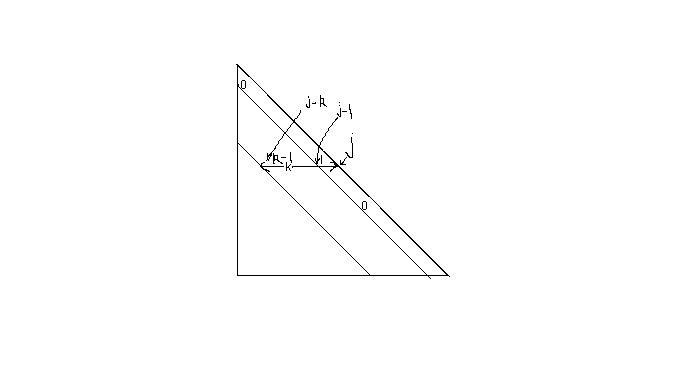
\includegraphics{bandedMatrix.png} A
very useful result: For Cholesky decomposition upon, the bandwidth of
\(A_n\) is k iff bandwidth of \(\Omega_n\) is \(k\).

%以上思路是,如果该阵是banded,那么经过cholesky变换以后,也应该是banded。

%突然想起来一点,an和cheng写的统计量构造是通过banded以后,那些应该为0的部分的和是否靠近0为点进行构造的。

%断点数据:抄完了 Bayesian Test and Selection for Bandwidth ofHigh-dimensional Banded Precision Matrices 的模型数据。
%下一步:要么继续写这篇文章的Hypothesis构造的算法,要么去抄An(2014)和
%Cheng(2017)模型构造以及构造细节。

Prior Distribution I'm not that concerned yet, however, should notice
that it is the conjugate prior. So the posterior distribution can be calculated in a closed form up to some normalizing constant.

Assumption is important for the proof of estimation consistency,
however, I regards this is ``not neccessary'' for the idea of method, so
omit in this review. But I think the explaination in Section 2.4 is good
and worth reading if involve the proof of consistency and other
property.

\hypertarget{main-result}{%
\subsubsection{Main result:}\label{main-result}}

\begin{enumerate}
\def\labelenumi{\arabic{enumi}.}
\item
  Bandwidth selection consistency
\item
  Consistency of One-Sample Bandwidth Test Here construct a Bayesian
  bandwidth test for the testing problem: \[
  H_0:k\leqslant k^* \ \textit{vs }\ H_1:k>k^* 
  \] This is a composite hypothesis. The hypothesis test is based on the
  Bayes factor \(B_{10}(X_n)\) defined by the \textbf{ratio of marginal
  likelihoods} , \[
  B_{10}(X_{n})=\frac{p(X_n|H_1)}{p(X_n|H_0)}
  \] Denote the prior under the hypothesis \(H_i\) as
  \(\pi_i(A_n,D_n,k)\) for \(i=0,1.\) Using prior \(\pi_0(k)\) and
  \(\pi_1(k)\) such that \[
  \begin{array} { l l } { \pi _ { 0 } ( k ) = C _ { 0 } ^ { - 1 } \pi ( k ) , \quad k = 0,1 , \ldots , k ^ { * } } \\ { \pi _ { 1 } ( k ) = C _ { 1 } ^ { - 1 } \pi ( k ) , \quad k = k ^ { \star } + 1 , \ldots , R _ { n } } \end{array}
  \] with \(C _ { 0 } = \sum _ { k = 0 } ^ { k ^ { * } } \pi ( k )\),
  \(C _ { 1 } = \sum _ { k = k ^ { * } + 1 } ^ { R _ { n } } \pi ( k )\).
  Then the Bayes factor (the statistic we construct for Hypothesis), is
  in analytic form, \[
  \begin{aligned} B _ { 10 } \left( \mathbf { X } _ { n } \right) & = \frac { \sum _ { k > k ^ { * } } \int p \left( \mathbf { X } _ { n } | \Omega _ { n } , k \right) \pi \left( \Omega _ { n } | k \right) \pi _ { 1 } ( k ) d \Omega _ { n } } { \sum _ { k \leq k ^ { * } } \int p \left( \mathbf { X } _ { n } | \Omega _ { n } , k \right) \pi \left( \Omega _ { n } | k \right) \pi _ { 0 } ( k ) d \Omega _ { n } } \\ & = \frac { \pi \left( k > k ^ { * } | \mathbf { X } _ { n } \right) } { \pi \left( k \leq k ^ { * } | \mathbf { X } _ { n } \right) } \times \frac { C _ { 0 } } { C _ { 1 } } \end{aligned}
  \] Consistency result: Under \(H_0:k\leq k^*\) \[
  B _ { 10 } \left( \mathbf { X } _ { n } \right) = O _ { p } \left( T _ { n , H _ { 0 } , k _ { 0 } , k ^ { * } } \right)
  \] Under \(H_1\) \[
  B _ { 10 } \left( \mathbf { X } _ { n } \right) ^ { - 1 } = O _ { p } \left( T _ { n , H _ { 1 } , k _ { 0 } , k ^ { * } } \right)
  \]
\end{enumerate}

Then is the method comparison between (An et al., 2014; Cheng et al.,
2017) and it's method. The mainly concern also is the consistency.

\begin{quote}
It is curious about the problem that how the test work, which means
significance under such bayes factor, such ratio?
\end{quote}

Quote from the arthor.

\begin{quote}
If \(H_0\) is true, \(B_{10}(Y)\) decreases at rate
\(O_p(e^{-c_0(k_2-k_1)})\) for some constant \(c_2>0\). On the other
hand, if \(H_1\) is true, \(B_{10}(Y)^{-1}\) decreases exponentially
with \(n(k_2-k_1)\beta^2_{min}\).
\end{quote}

So there should be some threshold for the ratio about ``decline the
null-hypothesis'' or the ``accept the alter-hypothesis'' like 1 or 0.95
something. Back to the form of the Bayes factor :
\(B_{10}(X_{n})=\frac{p(X_n|H_1)}{p(X_n|H_0)}\) ,if \(H_0\) is true,
then the denominator is larger than the numerator, bayes factor is
closer to 0. If \(H_1\) is true, then numerator \(p(X_n|H_1)\) should be
larger than the denominator. Then the inverse of the Bayes factor should
closer to 0.

Because as it says, (An et al., 2014; Cheng et al., 2017)'s result is
that the statistic they constructed is asymptotically under Normal
distribution, then it comes to the normal 95\%
hypothesis-test-framework. Need notice, the asymptotically achieve for
\(n \wedge p \rightarrow \infty\) rather than \(n \rightarrow \infty\).

\begin{quote}
Q : How the bayes factor linked with the Cholesky decomposition?
\end{quote}

\begin{quote}
A: Insider the analytic form of Bayes factor: \(p(X_n|\Omega_n,k)\) and
\(\pi(\Omega_n|k)\)
\end{quote}

\begin{enumerate}
\def\labelenumi{\arabic{enumi}.}
\setcounter{enumi}{2}
\tightlist
\item
  Two-Sample Bandwidth Test
\end{enumerate}

Problem: \[
\begin{array} { c } { X _ { 1 } , \ldots , X _ { n _ { 1 } } | \Omega _ { 1 n _ { 1 } } \stackrel { i . i . d . } { \sim } N _ { p } \left( 0 , \Omega _ { 1 n _ { 1 } } ^ { - 1 } \right)} \\ { Y _ { 1 } , \ldots , Y _ { n _ { 2 } } | \Omega _ { 2 n _ { 2 } } \stackrel { i . i . d } { \sim } N _ { p } \left( 0 , \Omega _ { 2 n _ { 2 } } ^ { - 1 } \right) } \end{array}
\] Interesting question: Test of equality between two bandwidths
\(k_1\)and \(k_2\). Hypothesis: \[
H _ { 0 } : k _ { 1 } = k _ { 2 },H _ { 1 } : k _ { 1 } \neq k _ { 2 }
\] Bayes factor: \[
B _ { 10 } \left( \mathbf { X } _ { n _ { 1 } } , \mathbf { Y } _ { n _ { 2 } } \right) = \frac { p \left( \mathbf { X } _ { n _ { 1 } } , \mathbf { Y } _ { n _ { 2 } } | H _ { 1 } \right) } { p \left( \mathbf { X } _ { n _ { 1 } } , \mathbf { Y } _ { n _ { 2 } } | H _ { 0 } \right) }
\]

\begin{quote}
How to investigate the posterior/probability under the \(H_1\)
\(p(X_{n1},Y_{n_2})\)?
\end{quote}

To answer this question, should deep in P14 the construction and the
specifying of the prior distribution inside \(a_{1,j}^{(k_0)}\) and
\(a_{1,j}^{(k_1)}\) for given \(k_0\) and \(k_1\).

Then the Bayes factor can be written as analytic form under the prior
given \[
B _ { 10 } \left( \mathbf { X } _ { n _ { 1 } } , \mathbf { Y } _ { n _ { 2 } } \right) = \frac { \sum _ { k _ { 1 } \neq k _ { 2 } } \pi \left( k _ { 1 } | \mathbf { X } _ { n _ { 1 } } \right) \pi \left( k _ { 2 } | \mathbf { Y } _ { n _ { 2 } } \right) } { \sum _ { k _ { 1 } = k _ { 2 } } \pi \left( k _ { 1 } | \mathbf { X } _ { n _ { 1 } } \right) \pi \left( k _ { 2 } | \mathbf { Y } _ { n _ { 2 } } \right) } \times R _ { n } ^ { - 1 }
\]

Use marginal posterior distribution to deal with the alternative
hypothesis \(k_1\neq k_2\). And arthor gives a theorem about the
consistency of such test.

\hypertarget{references}{%
\section*{References:}\label{references}}
\addcontentsline{toc}{section}{References:}

\hypertarget{refs}{}
\leavevmode\hypertarget{ref-An:2014jc}{}%
An, B., Guo, J., \& Liu, Y. (2014). Hypothesis testing for band size
detection of high-dimensional banded precision matrices.
\emph{Biometrika}, \emph{101}(2), 477--483.

\leavevmode\hypertarget{ref-Banerjee:2015ex}{}%
Banerjee, S., \& Ghosal, S. (2015). Bayesian structure learning in
graphical models. \emph{Journal of Multivariate Analysis}, \emph{136},
147--162.

\leavevmode\hypertarget{ref-Cheng:2017jh}{}%
Cheng, G., Zhang, Z., \& Zhang, B. (2017). Test for bandedness of
high-dimensional precision matrices, 1--20.

\leavevmode\hypertarget{ref-Johnstone:tc}{}%
Johnstone, I. M., manuscript, A. L. U., \& 2004. (n.d.). Sparse
principal components analysis. \emph{Pdfs.semanticscholar.org}.

\leavevmode\hypertarget{ref-Lee:2017uq}{}%
Lee, K., \& Lee, J. (2017). Estimating Large Precision Matrices via
Modified Cholesky Decomposition. \emph{arXiv.org}. Retrieved from
\url{http://arxiv.org/abs/1707.01143v1}

\leavevmode\hypertarget{ref-Lee:2018vj}{}%
Lee, K., \& Lin, L. (2018). Bayesian Test and Selection for Bandwidth of
High-dimensional Banded Precision Matrices. \emph{arXiv.org}. Retrieved
from \url{http://arxiv.org/abs/1804.08650v1}

\leavevmode\hypertarget{ref-Pan:2017il}{}%
Pan, J., \& Pan, Y. (2017). jmcm: An RPackage for Joint Mean-Covariance
Modeling of Longitudinal Data. \emph{Journal of Statistical Software},
\emph{82}(9), 1--29.

\leavevmode\hypertarget{ref-Pourahmadi:2000fs}{}%
Pourahmadi, M. (2000). Maximum likelihood estimation of generalised
linear models for multivariate normal covariance matrix.
\emph{Biometrika}, \emph{87}(2), 425--435.


\end{document}
